%%%%%%%%%%%%%%%%%%%%%%%%%%%%%%%%%%%%%%%%%
% Bachelor/Master Thesis 
% LaTeX Template
% Version 2.5 (27/8/17)
%
% This template was downloaded from:
% http://www.LaTeXTemplates.com
%
% Version 2.x major modifications by:
% Vel (vel@latextemplates.com)
%
% This template is based on a template by:
% Steve Gunn (http://users.ecs.soton.ac.uk/srg/softwaretools/document/templates/)
% Sunil Patel (http://www.sunilpatel.co.uk/thesis-template/)
%
% Template license:
% CC BY-NC-SA 3.0 (http://creativecommons.org/licenses/by-nc-sa/3.0/)
%
%%%%%%%%%%%%%%%%%%%%%%%%%%%%%%%%%%%%%%%%%

%----------------------------------------------------------------------------------------
%	PACKAGES AND OTHER DOCUMENT CONFIGURATIONS
%----------------------------------------------------------------------------------------

\documentclass[
11pt, % The default document font size, options: 10pt, 11pt, 12pt
oneside, % Two side (alternating margins) for binding by default, uncomment to switch to one side
english, % ngerman for German
singlespacing, % Single line spacing, alternatives: onehalfspacing or doublespacing
%draft, % Uncomment to enable draft mode (no pictures, no links, overfull hboxes indicated)
%nolistspacing, % If the document is onehalfspacing or doublespacing, uncomment this to set spacing in lists to single
%liststotoc, % Uncomment to add the list of figures/tables/etc to the table of contents
%toctotoc, % Uncomment to add the main table of contents to the table of contents
%parskip, % Uncomment to add space between paragraphs
%nohyperref, % Uncomment to not load the hyperref package
headsepline, % Uncomment to get a line under the header
%chapterinoneline, % Uncomment to place the chapter title next to the number on one line
%consistentlayout, % Uncomment to change the layout of the declaration, abstract and acknowledgements pages to match the default layout
]{BachelorMasterThesis} % The class file specifying the document structure

\usepackage[utf8]{inputenc} % Required for inputting international characters
\usepackage[T1]{fontenc} % Output font encoding for international characters

\usepackage{mathpazo} % Use the Palatino font by default

\usepackage[backend=bibtex,style=alphabetic,natbib=true]{biblatex} % Use the bibtex backend with the authoryear citation style (which resembles APA)

\usepackage[autostyle=true]{csquotes} % Required to generate language-dependent quotes in the bibliography

% MY CUSTOM SETTINGS
\usepackage{minted} % code snippets
\usepackage{soul} % strikethrough text
\usepackage{enumitem} % formatting enumerated lists
\usepackage{ulem} % underlining text
\usepackage{xcolor} % text color
\usepackage{pgfplots}

% space between footnotes
\setlength{\footnotesep}{0.4cm}
% space between text body and footnotes
\setlength{\skip\footins}{1cm}

% my bibliography
\addbibresource{./thesis.bib}

%----------------------------------------------------------------------------------------
%	MARGIN SETTINGS
%----------------------------------------------------------------------------------------

\geometry{
	paper=a4paper, % Change to letterpaper for US letter
	inner=2.5cm, % Inner margin
	outer=3.8cm, % Outer margin
	bindingoffset=.5cm, % Binding offset
	top=1.5cm, % Top margin
	bottom=1.5cm, % Bottom margin
	%showframe, % Uncomment to show how the type block is set on the page
}

%----------------------------------------------------------------------------------------
%	THESIS INFORMATION
%----------------------------------------------------------------------------------------

\thesistitle{Compile time semantic analysis and verification of conceptual models in application to transactional business information systems} % Your thesis title, this is used in the title and abstract, print it elsewhere with \ttitle
\supervisor{Oles \textsc{Hodych}, PhD} % Your supervisor's name, this is used in the title page, print it elsewhere with \supname
\examiner{} % Your examiner's name, this is not currently used anywhere in the template, print it elsewhere with \examname
\degree{Bachelor of Science} % Your degree name, this is used in the title page and abstract, print it elsewhere with \degreename
\author{Vladyslav \textsc{Bilyk}} % Your name, this is used in the title page and abstract, print it elsewhere with \authorname
\addresses{} % Your address, this is not currently used anywhere in the template, print it elsewhere with \addressname

\subject{} % Your subject area, this is not currently used anywhere in the template, print it elsewhere with \subjectname
\keywords{} % Keywords for your thesis, this is not currently used anywhere in the template, print it elsewhere with \keywordnames
\university{\href{http://www.ucu.edu.ua}{Ukrainian Catholic University}} % Your university's name and URL, this is used in the title page and abstract, print it elsewhere with \univname
\department{\href{http://department.university.com}{Faculty of Applied Sciences}} % Your department's name and URL, this is used in the title page and abstract, print it elsewhere with \deptname
\group{\href{http://researchgroup.university.com}{Department of Computer Sciences}} % Your research group's name and URL, this is used in the title page, print it elsewhere with \groupname
\faculty{\href{http://faculty.university.com}{}} % Your faculty's name and URL, this is used in the title page and abstract, print it elsewhere with \facname

\AtBeginDocument{
\hypersetup{pdftitle=\ttitle} % Set the PDF's title to your title
\hypersetup{pdfauthor=\authorname} % Set the PDF's author to your name
\hypersetup{pdfkeywords=\keywordnames} % Set the PDF's keywords to your keywords
}

\begin{document}

\frontmatter % Use roman page numbering style (i, ii, iii, iv...) for the pre-content pages

\pagestyle{plain} % Default to the plain heading style until the thesis style is called for the body content

%----------------------------------------------------------------------------------------
%	TITLE PAGE
%----------------------------------------------------------------------------------------

\begin{titlepage}
\begin{center}

\vspace*{.04\textheight}
{\scshape\LARGE \univname\par}\vspace{1.5cm} % University name
\textsc{\Large Bachelor Thesis}\\[0.3cm] % Thesis type

\HRule \\[0.4cm] % Horizontal line
{\LARGE \bfseries \ttitle\par}\vspace{0.4cm} % Thesis title
\HRule \\[1.5cm] % Horizontal line
 
\begin{minipage}[t]{0.4\textwidth}
\begin{flushleft} \large
\emph{Author:}\\
%\href{http://www.johnsmith.com}
{\authorname} % Author name - remove the \href bracket to remove the link
\end{flushleft}
\end{minipage}
\begin{minipage}[t]{0.4\textwidth}
\begin{flushright} \large
\emph{Supervisor:} \\
%\href{http://www.jamessmith.com}
{\supname} % Supervisor name - remove the \href bracket to remove the link  
\end{flushright}
\end{minipage}\\[3cm]
 
\large \textit{A thesis submitted in fulfillment of the requirements\\ for the degree of \degreename}\\[0.3cm] % University requirement text
\textit{in the}\\[0.4cm]
\groupname\\\deptname\\[1cm] % Research group name and department name
 
\smallskip

\includegraphics[height=5cm]{UCU-Apps.png} % University/department logo - uncomment to place it

\smallskip
{\large Lviv 2022}\\[4cm] % Date
 
\vfill
\end{center}
\end{titlepage}

%----------------------------------------------------------------------------------------
%	DECLARATION PAGE
%----------------------------------------------------------------------------------------

\begin{declaration}
\addchaptertocentry{\authorshipname} % Add the declaration to the table of contents
\noindent I, \authorname, declare that this thesis titled, \enquote{\ttitle} and the work presented in it are my own. I confirm that:

\begin{itemize} 
\item This work was done wholly or mainly while in candidature for a research degree at this University.
\item Where any part of this thesis has previously been submitted for a degree or any other qualification at this University or any other institution, this has been clearly stated.
\item Where I have consulted the published work of others, this is always clearly attributed.
\item Where I have quoted from the work of others, the source is always given. With the exception of such quotations, this thesis is entirely my own work.
\item I have acknowledged all main sources of help.
\item Where the thesis is based on work done by myself jointly with others, I have made clear exactly what was done by others and what I have contributed myself.\\
\end{itemize}
 
\noindent Signed:\\
\rule[0.5em]{25em}{0.5pt} % This prints a line for the signature
 
\noindent Date:\\
\rule[0.5em]{25em}{0.5pt} % This prints a line to write the date
\end{declaration}

\cleardoublepage

%----------------------------------------------------------------------------------------
%	QUOTATION PAGE
%----------------------------------------------------------------------------------------

%\vspace*{0.2\textheight}


%\noindent\enquote{\itshape To those human beings who are of any concern to me I wish suffering, desolation, sickness, ill-treatment, indignities—I wish that they should not remain unfamiliar with profound self-contempt, the torture of self-mistrust, the wretchedness of the vanquished: I have no pity for them, because I wish them the only thing that can prove today whether one is worth anything or not—that one endures.}\bigbreak

%\hfill Friedrich Nietzsche

%----------------------------------------------------------------------------------------
%	ABSTRACT PAGE
%----------------------------------------------------------------------------------------

\begin{abstract}
\addchaptertocentry{\abstractname} % Add the abstract to the table of contents
The essential complexity of software, manifested in the size of software entities, makes it a daunting task for programmers to keep comprehensive knowledge of the domain in their minds. The accidental difficulty is the lack of appropriate tools for efficient domain discoverability during design time of software systems, as well as construction of reliable and evolvable models.
\end{abstract}

%----------------------------------------------------------------------------------------
%	ACKNOWLEDGEMENTS
%----------------------------------------------------------------------------------------

\begin{acknowledgements}
\addchaptertocentry{\acknowledgementname} % Add the acknowledgements to the table of contents
\n

\noindent I would like to thank the following for their help in connection with this thesis:

\n\n\n

\noindent My thesis supervisor, Oles Hodych, for his valuable feedback and support throughout this project.

\n\n\n

\noindent The software engineering team at Trident Genesis for participating in the experiments.

\n\n\n

\noindent Armed Forces of Ukraine for protecting our country and our freedom.
\end{acknowledgements}

%----------------------------------------------------------------------------------------
%	LIST OF CONTENTS/FIGURES/TABLES PAGES
%----------------------------------------------------------------------------------------

\tableofcontents % Prints the main table of contents

\listoffigures % Prints the list of figures

%\listoftables % Prints the list of tables

%----------------------------------------------------------------------------------------
%	ABBREVIATIONS
%----------------------------------------------------------------------------------------

\begin{abbreviations}{ll} % Include a list of abbreviations (a table of two columns)
\textbf{APT} & \textbf{A}nnotation \textbf{P}rocessing \textbf{T}ool\\
\textbf{JDK} & \textbf{J}ava \textbf{D}evelopment \textbf{K}it\\
\textbf{AST} & \textbf{A}bstract \textbf{S}yntax \textbf{T}ree\\
\textbf{JLS} & \textbf{J}ava \textbf{L}anguage \textbf{S}pecification\\
\textbf{ORM} & \textbf{O}bject/\textbf{R}elational \textbf{M}apping\\
\textbf{DDD} & \textbf{D}omain-\textbf{D}riven \textbf{D}esign\\
\end{abbreviations}

%----------------------------------------------------------------------------------------
%	PHYSICAL CONSTANTS/OTHER DEFINITIONS
%----------------------------------------------------------------------------------------

%\begin{constants}{lr@{${}={}$}l} % The list of physical constants is a three column table
%
%% The \SI{}{} command is provided by the siunitx package, see its documentation for instructions on how to use it
%
%Speed of Light & $c_{0}$ & \SI{2.99792458e8}{\meter\per\second} (exact)\\
%%Constant Name & $Symbol$ & $Constant Value$ with units\\
%
%\end{constants}

%----------------------------------------------------------------------------------------
%	SYMBOLS
%----------------------------------------------------------------------------------------

%\begin{symbols}{lll} % Include a list of Symbols (a three column table)
%
%$a$ & distance & \si{\meter} \\
%$P$ & power & \si{\watt} (\si{\joule\per\second}) \\
%%Symbol & Name & Unit \\
%
%\addlinespace % Gap to separate the Roman symbols from the Greek
%
%$\omega$ & angular frequency & \si{\radian} \\
%
%\end{symbols}

%----------------------------------------------------------------------------------------
%	DEDICATION
%----------------------------------------------------------------------------------------

%\dedicatory{For/Dedicated to/To my\ldots} 

%----------------------------------------------------------------------------------------
%	THESIS CONTENT - CHAPTERS
%----------------------------------------------------------------------------------------

\mainmatter % Begin numeric (1,2,3...) page numbering

\pagestyle{thesis} % Return the page headers back to the "thesis" style

% Include the chapters of the thesis as separate files from the Chapters folder
% Uncomment the lines as you write the chapters

\chapter{Introduction}

% object, area, goal
An important piece of work in the information systems field by Antoni Olive \cite{CMofIS} defines the term \textit{conceptual modeling} as the activity of describing and structuring the general knowledge a particular information system needs to know.
The main objective of conceptual modeling is to obtain that description, which is called a \textit{conceptual schema}.
Conceptual modeling is an important part of requirements engineering, the first and most important phase in the development of an information system.
However, any information system will invariably undergo modification, either due to the demands of its users or as a result of a change in the nature of the information itself or for other reasons.
Therefore, one of the most important properties of information systems is evolvability.

\n

%It is often the case that a description of a conceptual schema needs to be represented in a system. 
%However, not in the form of source code, but contained in the source code.
An ability to access and process the information about a conceptual schema programmatically at runtime is widely used by various technologies for automation of otherwise complex and error-prone software engineering tasks.
For example, Object-Relational Mapping (ORM)\footnote{Object-Relational Mapping is a technique used to interact with a database through an interface in object-oriented paradigm.} technologies automate mapping between two representations of a conceptual schema: expressed in OOP terms as classes and expressed in terms of a relational database.
This information is a structured representation of a conceptual schema, which we shall refer to as \textit{meta-model}.
Although accessible at runtime, such meta-models also need to be made available to software engineers at design time.
The information provided by meta-model is called \textit{metadata}.
Since this meta-level information is also a part of a system it is desirable for it to be evolvable as well.
Moreover, due to the fact that a meta-model reflects the structure of a conceptual schema, it must be consistent with it.
Ideally, a meta-model would always be automatically updated to match the structure of a conceptual schema.

\n

The aim of this research is to develop a technology for compile time semantic analysis that would capture the description of conceptual models in a form of metadata directly represented in the source code. 
We outline the following objectives:
\begin{enumerate}
    \item Improve \textit{domain modeling} efficiency and provide advanced \textit{domain discoverability} features at design time.
    \item Improve system reliability and ensure correctness of references to domain models at compile time.
    \item Improve system evolvability.
\end{enumerate}

The key result of this research is the developed technology itself -- an approach to achieve the stated objectives.

\section{Domain modeling}
Any software system aims to address a specific problem.
The area surrounding this problem is known as the problem domain. \textit{Domain modeling} is a form of conceptual modeling commonly used in software engineering.
Its aim is to construct a \textit{domain model} -- a structured representation of the problem domain with a description of core concepts and their relationships.
We define \textit{domain discoverability} as the ability to \textit{discover} the domain model, that is, to inspect the conceptual schema of the domain.
We later show that domain discoverability can be limited by the programming language used to write the software.

\n

% rewrite in terms of conceptual modeling of information systems + a constant need for change
Efficient software engineering requires a certain kind of knowledge to be present in the mind of a software engineer. 
Peter Naur \cite{naur} conveyed an insightful idea of Theory Building View of programming, stating that a program is a shared mental construct that lives in the minds of the people who work on it.
Therefore, the programmer possessing the theory is able to respond constructively to any demand for a modification of the program.
The same can be said about domain modeling where the general knowledge of the domain needs to be present at all times in order to develop correct models.
However, that might prove to be a difficult task for a domain of significant size, requiring the software engineers to frequently brush up their knowledge of the target domain through the use of a secondary source of information, such as documentation or source code of the software.
In order to tackle this difficulty many supporting tools have been developed. For example, modern IDEs\footnote{Integrated Development Environment (IDE) is software that combines common developer tools into a single graphical user interface.} come with a handful of advanced features, such as code auto-completion, which is a practical way of enhancing domain discoverability.

\n

Brooks \cite{brooks} defines two kinds of complexity involved in the process of software construction: essential and accidental.
Essential complexity stems from the inherent properties of software, such as the size of software systems, conformity to other interfaces, changeability and invisibility (inability to be visualized).
Accidental complexity is manifested in any activity that engages in representation of conceputal software structures in programming languages and mapping of those structures onto machine languages within space and speed constraints.
Among past breakthroughs in solving accidental difficulties are: high-level programming languages, time-sharing systems and unified programming environments.
Following Brooks’s excerpt on time-sharing which he views as an attack on a specific accidental difficulty -- interruption of consciousness due to a need to call for compilation and execution, which might result in the decay of grasp of all that is going on in a complex system -- our main hypothesis is that the lack of programming language-level metamodeling facilities with advanced design-time domain discoverability features is the same kind of difficulty with negative effects of similar nature.

\section{System reliability}
% informal reasoning, cite Out of the Tar Pit
Reliability of a system is its ability to perform a given task in an expected way without causing errors.
In order to build reliable systems it is important to understand those systems.
Moseley \& Marks \cite{moseley} identified two widely-used approches to understanding systems: \textit{testing} and \textit{informal reasoning}; with an emphasis on the importance of the latter.
Informal reasoning is an attempt to understand the system by examining it from the inside.
Its importance was explained by Moseley \& Marks by the fact that improvements in informal reasoning lead to \textit{less errors being created}, as opposed to improvements in testing that lead only to \textit{more errors being detected}.
One of the desirable properties of testing is high code coverage, which is a measure of the amount of source code of a program that was executed, hence covered, during testing.
However, for systems of significant size, characterized by large code volume with complex structure, testing is usually a time consuming process.
No guarantees can be given that a failing test will not occur at the very end of the whole process.
Because of this, understanding systems through testing is also more time-consuming.
Therefore, it is preferable to focus on ways of improving informal reasoning.

\n

When we examine a system from the inside we do it at design time, that is, during the phase of system construction.
For example, reasoning about the source code of a system's component is an activity carried out at design time.
Modern IDEs blur the line between design time and compile time, seemlessly integrating the compilation process into design time in order to increase developer productivity.
This allows software engineers to benefit from messages signaled by a compiler, making a great contribution to improvements in informal reasoning.
Therefore, delegating as much system validation as possible to a compiler will result into more reliable systems.

\section{System evolvability}
% link this to "informal reasoning" (out of the tar pit)
All systems are prone to change, especially the successful ones.
This is due to the fact that software that is found to be useful is often pushed to its limits by its users who invent new uses for it.
Change management thus plays an essential role in the lifecycle of a software system.
Whenever a change is introduced to the domain model, all parts of a system that interact with the changed component must be verified and modified if necessary.
While the verification is usually covered by automated tests, the modification of related components has to be carried out by a software engineer.
In order to ensure that the latest change is adopted correctly a software engineer must know the exact locations of those components in the source code.
Once again, this can be a difficult task when working with a large system and that is why the role of a compiler is critical, for it can inform the software engineer of those places in the source code.

\n

The underlying assumption is that software is being developed in a compile time safe manner.
However, given the general purpose nature of modern programming languages, this assumption is not always true.
There is a lack of a language-level abstraction that could be used as domain model metadata, that carries type information, to reference the conceptual model.
This limitation forces software engineers to use textual string representations instead that are "hard-coded" into the program.
This is known to be unreliable because a compiler can't validate the contents of a string, thus a program deemed valid by a compiler might contain incorrect metadata that results in a runtime error.
Although, were the metadata represented in the form of a meta-model instead, all rules of compile time validation would be applicable to it.
Moreover, any modification to the domain model would be reflected in the meta-model.
Therefore, it would be possible to efficiently track the related components in need of modification at design time due to messages signaled by a compiler.

\n

To illustrate a possible case where a meta-model might be required we provide the following example.
A simple example of a situation where domain model metadata is required is illustrated in the following code snippet that constructs a query to a database:

\begin{listing}[H]
    \begin{minted}{java}
    class Customer {
        private String name;
        private int age;
    }
    \end{minted}
    \caption{A java class for a \texttt{Customer} concept.}
    \label{lst:intro-customer}
\end{listing}


\begin{listing}[H]
    \begin{minted}{java}
    String query = "SELECT name FROM customers WHERE age >= 21;";
    \end{minted}
    \caption{SQL query with hard-coded metadata that fetches the names of all customers of age over 21.}
    \label{lst:intro-sql-raw}
\end{listing}

The problem with this code is that it uses "hard-coded" metadata.
A compiler can't tell whether \texttt{name} is a part of the \texttt{Customer} concept.
It also has no way of verifying whether \texttt{customers} is a valid database table.
As a result, this code is unreliable and difficult to maintain.
It is easy to imagine that some time in the future the conceptual schema might change leading to the \texttt{Customer} concept no longer having the attribute \texttt{name}, but \texttt{fullName} instead.
Consequently, each such occurence of hard-coded metadata must be manually located throughout the whole system.

\n

It is true that using raw strings to construct SQL queries is a bad practice and alternative approaches have been developed, such as ORM frameworks.
However, the core issue still remains unsolved, as demonstrated by the following example.

\begin{listing}[H]
    \begin{minted}{java}
    QueryModel<Customer> query = select(Customer.class).where()
        .prop("age").gt().val(21)
        .yield().prop("name")
        .model();
    \end{minted}
    \caption{SQL query from \ref{lst:intro-sql-raw} expressed using an ORM framework.}
    \label{lst:intro-eql}
\end{listing}

The \texttt{"age"} and \texttt{"name"} strings still must be used to refer to \texttt{Customer} attributes.

\smallskip

Now, consider an approach utilizing a meta-model:

\begin{listing}[H]
    \begin{minted}{java}
    QueryModel<Customer> query = select(Customer.class).where()
        .prop(Customer_.age).gt().val(21)
        .yield().prop(Customer_.name)
        .model();
    \end{minted}
    \caption{SQL query from \ref{lst:intro-eql} using a meta-model.}
    \label{lst:intro-sql-meta}
\end{listing}

Here \texttt{Customer\_} is a meta-model class. 
It guarantees that the database query is constructed in a compile time safe manner, since a change to the domain model is immediately reflected in the meta-model.
In case a breaking change took place, an appropriate compilation error would follow.

\section{Technical approach}
Taking into account the widespread adoption and use of object-oriented programming in domain-driven design, we focus on the Java programming language in particular.
Since Java language specification does not support class meta-models, we provide our own implementation of a meta-model generation mechanism. 
The implementation is based on a feature of Java -- annotations, supplemented by annotation processing -- an ability to process annotations at compile time.

\n

The implementation we provide is designed with a particular software development technology in mind – Trident Genesis (TG). The choice was made to integrate the implementation with the surrounding framework in order to make the development process manageable in terms of time, and, given its experimental nature, it was preferable to narrow down the scope of application, while making it practical. This choice does not invalidate a general nature of the research.

\n
Trident Genesis (TG) is a software development technology, which has been developed by Fielden Management Services Pty. Ltd (Australia).

\n

TG fits well into the definition of domain-driven development, as it shares the common language of domain modeling, speaking in terms of domain entities and their relationships.

\section {Qualitative research}
In order to assess the extent to which the stated objectives were achieved the experimental component of this work is carried out by employing an approach of qualitative research.
The applictation of qualitative reserach to the field of software engineering is discussed by Hazzan \& Dubinsky \cite{hazzan}.

\n

The conducted experiments involve a focus group of select software engineers from the industry, who are practicing domain-driven development as their main software design approach, making them ideal candidates to test our main hypotheses.
We use a questionnaire as a main data gathering tool.

\n

Richard Pawson \cite{pawson}'s work is one great example of an application of qualitative research methods to the field of software engineering.

\section{Structure}

This work is structured in the following way: 

\n

\noindent Chapter 2 goes into depth about key concepts and provides the necessary background for the rest of the paper.

\n

\noindent Chapter 3 discusses related work, comparing the approaches employed. Each approach is examined in great detail with its strengths and limitations outlined.

\n

\noindent Chapter 4 provides a detailed description of the implementation. It discusses the developed algorithm step-by-step with attached illustrations and examples.

\n

\noindent Chapter 5 describes the experiment. It includes a display of the questionnaire contents and answers of the participants.

\n

\noindent Chapter 6 discusses future work that encompasses a general framework independent approach and draws on shortcomings of the implementation.

\chapter{Background}
This chapter covers the background for the fundamental concepts in this work in order to provide a deeper understanding of the research area and prepare the reader for the discussion of related work and the explanation of implementation details.
We start with the topic of conceptual modeling in the context of software systems.
Then, we introduce the approach of \textit{domain-driven design}, which is followed by the description of the Java programming language and its application to this research.

\section{Conceptual modeling of software systems}
Conceptual modeling is an integral part of software construction.
In software engineering field the term "conceptual schema" is often associated with the world of relational database management systems (RDBMS).
A conceptual schema describes the structure of a database from a high-level perspective.
More specifically, it identifies the core concepts and classifies them into tables, which contain columns that stand for the attributes of a concept.
A conceptual schema does not include any internal details about a database.

\n

For example, in a banking system domain, the conceptual schema might describe concepts such as \textit{banking accounts and transactions}, as well as their relationship.
One common language for expressing conceptual schemas is UML.
Consider the banking example illustrated in the following UML class diagram:

\begin{figure}[H]\centering
    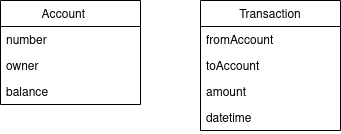
\includegraphics[scale=0.65]{images/banking.drawio.png}
    \caption{UML class diagram for a simplified banking domain}\label{fig:bank}
\end{figure}

Here the conceptual schema consists of two domain entities.
Both of them are characterized by specific attributes that describe their structure.
And it is a common occurence that the underlying structure of an entity might undergo some kind of modification.
For example, consider the diagram below that introduces a new attribute to the \texttt{Account} entity, namely, its creation date:

\begin{figure}[H]\centering
    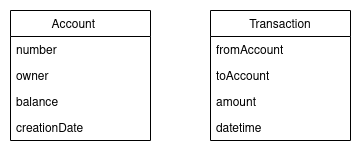
\includegraphics[scale=0.65]{images/banking1.drawio.png}
    \caption{UML class diagram illustrating an additive change to the conceptual model}\label{fig:bank1}
\end{figure}

\n

Modifications on a conceptual level, such as these, must be performed with caution, since they are fundamental in their nature.
This means that every part of the system that interacts with a modified concept should be taken into account during verification.
However, a simple additive change, as illustrated by the example, is relatively safe.
Consider another example showing an existing attribute of \texttt{Account} being modified:

\begin{figure}[H]\centering
    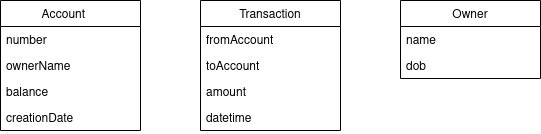
\includegraphics[scale=0.65]{images/banking2.drawio.png}
    \caption{UML class diagram illustrating a breaking change to the conceptual model}\label{fig:bank2}
\end{figure}

The \texttt{ownerName} attribute of \texttt{Account} has been replaced by \texttt{owner}.
The \texttt{Owner} concept has also been included in the diagram to provide the necessary context.
This kind of change is often refered to as a \textit{breaking change}, since it might "break" the system if any of its components were using the modified part.
Given that prior to this change the \texttt{ownerName} attribute was a simple textual representation, any part of the system that was refering to this attribute must be modified accordingly.
Ideally, after a modification has taken place, the system would be automatically validated to detect any errors that might have resulted from the modification.
In our example it would be expected that the validation mechanism reports that the \texttt{Account} concept does not define an attribute \texttt{ownerName}, if it was used prior to the modification.

%\n
%
%However, the world of software systems is not perfect.
%Database querying mechanisms work under the assumption that their input is consistent with the actual conceptual schema.
%If incorrect input is supplied, it will most likely cause the system to fail when it is already running or being tested.

\section{Domain-driven design and its terminology}
Domain-driven design, a term coined by Eric Evans \cite{ddd}, is an approach to conceptual modeling of a specific business domain.
Its main aim is construction of a domain model, which translates to a conceptual model of the domain.
At the heart of domain-driven design one of the basic building blocks is an \textit{entity}, that is, a domain object defined primarily by its identity.
We use the term \textit{entity} interchangeably with the term \textit{concept} assuming that the concept has an identity. 
Every entity is characterized (but not necessarily identified) by its \textit{properties} in the same way that every concept is characterized by its \textit{attributes}.

\section{Java programming language}
Java \cite{java} is a compiled, high-level, class-based, object-oriented programming language.
In practice it is often used to implement domain-driven software systems, mapping domain objects to Java classes.
Fields of a Java class are used to represent properties of an entity.
For example, the domain from \ref{fig:bank} could be modeled in the following way:

\begin{listing}[H]
    \begin{minted}{java}
        class Account {
            private int number;
            private String ownerName;
            private float balance;
        }

        class Transaction {
            private Account fromAccount;
            private Account toAccount;
            private float amount;
            private DateTime datetime;
        }
    \end{minted}
    \caption{The domain illustrated in \ref{fig:bank} modeled in Java.}
    \label{lst:bank}
\end{listing}

\section{Java reflection}
The reflection capabilities of Java are briefly discussed in this section, since they are often mentioned alongside with the terms \textit{metadata} and \textit{metaprogramming}.
In contrast with other compiled languages, such as C, Java is characterized by its sophisticated runtime mechanism that provides dynamic capabilities, such as reflection and code modification.
Reflection, in particular, makes metaprogramming possible, which allows the program to use other programs, itself included, as data.
For example, using reflection it is possible to obtain the type of a class field by its name:

\begin{minted}{java}
class Person {
    private Animal pet;
}

Person.class.getDeclaredField("pet").getType()); // class Animal
\end{minted}

Although this is a powerful programming technique that allows runtime type introspection to take place, it can not be used to treat the source code of a program as data at compile time.
The runtime nature of reflection indicates that reflection operates on objects constructed from compiled code.
This means that metadata obtained by using reflection exists only at runtime of the system, which is out of compiler's scope.

\section{Java annotations}
The Java Language Specification \cite{jls} defines a special construct – annotations – that provides data about a program that is not part of the program itself, in other words, it has no direct effect on the operation of code that is annotated.
Annotations may be used to provide additional information to the compiler or to be interpreted during runtime of the program.
We focus on the compile time processing of annotations.
As an example, the \texttt{@Deprecated} annotation can be used to tell the compiler to generate warnings in places where the annotated element is used.

\begin{minted}[escapeinside=||]{java}
class Transformer {
    @Deprecated
    public static boolean isTransformable(Item item) {
        ...
    }
}

// warn: the method Transformer.isTransformable(Item) is deprecated
Transformer.|\st{isTransformale}|(someItem);
\end{minted}

The annotated method can still be used as if there was no annotation, but the warning makes it clear to a software engineer that the method is no longer supported and its usage is discouraged.

\section{Annotation processing}
Annotation processing, as its name implies, is a mechanism for processing annotations in the source code at compile time.
An important distinction from the previously mentioned concept of reflection is that the input of an annotation processor is an AST\footnote{Abstract syntax tree is a tree-like data structure used by the compiler to represent the structure of program source code.} constructed from the source code.

\n

The \texttt{@Deprecated} annotation in the example above is one of the Java built-in annotations. It gets processed by a built-in annotation processor that is a part of the Java compiler.

\n

The standard library of Java includes a common interface to all annotation processors, so software engineers can provide their own implementations, and instruct the compiler to use them.
Apart from issuing compile time warnings and errors, annotation processing supports programmatic generation of new code.
The following figure depicts the compilation process of javac\footnote{Java compiler included in the JDK from Oracle}.

\begin{figure}[H]\centering
    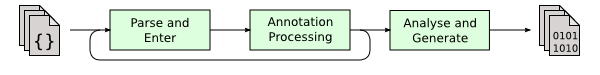
\includegraphics[scale=0.8]{images/javac-flow.png}
    \caption[Compilation process of javac]{Compilation process of \texttt{javac}}\label{fig:javac-flow}
\end{figure}

Java compilation process can be broken down into the following steps:

\begin{enumerate}
    \item The input source files are parsed to build a syntax tree.
    \item All appropriate annotation processors are run until no new files are generated.
    \item The syntax tree is analyzed to generate byte-code.
\end{enumerate}

It is important to mention that step 1 may differ across compiler implementations. The main difference lies in the input of a compiler. There is a notion of incremental compilation, which provides an ability to limit the number of source files that are passed as input to the compiler. As opposed to traditional compilation that requires the whole set of source files to be recompiled, an incremental compiler’s input is limited to that portion of the program that was modified.

\n

The built-in annotation processing API in Java has a rich collection of types that model the source language itself, equipping programmers with a powerful abstraction to analyze the syntax tree.\footnote{\texttt{javax.annotation.processing -- \url{https://docs.oracle.com/javase/8/docs/api/javax/annotation/processing/package-summary.html}}}

%\begin{relatedwork}

% add chapter to table of contents
%\addchaptertocentry{Related Work}

\chapter{Related work}

\section{C\# nameof}

    C\# has a \texttt{nameof} expression that is used to obtain the name of a program element as a constant string.\footnote{\href{https://docs.microsoft.com/en-us/dotnet/csharp/language-reference/operators/nameof}{\texttt{nameof}}} 

\begin{minted}{csharp}
using System.Collections.Generic;

class Program {
    static void Main() {
        string s1 = nameof(Program);                     // "Program"
        string s2 = nameof(Program.InstanceMethod);      // "InstanceMethod"
        string s3 = nameof(System.Collections.Generic);  // "Generic"
        // Invalid
        string s4 = nameof(int);               // Keywords not permitted
    }
    void InstanceMethod() { }
}
\end{minted}

% TODO
The result of the \texttt{nameof} expression is evaluated at compile time, meaning that \texttt{nameof(x)} if \texttt{x} is legal input is replaced by \texttt{"x"} in the resulting bytecode of the program. Our interest is drawn, however, to the use of property literals as string constants. And indeed nameof accepts class properties as input:

\begin{minted}{csharp}
class Book {
    public string title { get; set; }
}
nameof(Book.title) // "title"
\end{minted}

This is quite an effective way of using property literals as constant strings and it satisfies the compile time model correctness property. There are, however, several limitations to this approach, which are demonstrated below with provided examples:

\begin{enumerate}
    \item The \texttt{nameof} expression cannot be applied to class members with restricted access, such as private members. Although we consider this a limitation, the example above, which makes use of C\# Properties\footnote{\href{https://docs.microsoft.com/en-us/dotnet/csharp/programming-guide/classes-and-structs/properties}{C\# properties}}, is not constrained by it.

    \item The nameof expression always returns a simple name of its input, that is, the resulting name is not fully-qualified. This was demonstrated in the first code snippet:
\begin{minted}{csharp}
    string s3 = nameof(System.Collections.Generic);  // "Generic"
\end{minted}

\end{enumerate}

This limitation requires additional functionality to be implemented to concatenate the resulting string constants into a proper representation of the dot-notation.

\begin{minted}{csharp}
class Book {
    public string title { get; set; }
    public Author author { get; set; };
}
class Author {
    public string fullName { get; set; }
}

// "author.fullName"
DotNotation.Of(nameof(Book.author), nameof(Book.author.fullName));

class DotNotation {
    public static string Of(params string[] names) {
            return String.Join(".", names);
    }
}
\end{minted}

\texttt{Book.author.fullName} is used instead of simply \texttt{Author.fullName} to satisfy the compile time safety requirement. If the latter was used and the conceptual schema was changed leading to the type of \texttt{Book.author} not being \texttt{Author} anymore, but instead a value object or another entity that doesn’t have the property \texttt{fullName}, a run-time error would occur at the moment of the dot-notation being used (to fetch some data from a database, for example). Consequently, this results in an unintuitive and overly verbose code.

\section{Java nameof hack}

While the java programming language specification does not define property literals or an expression similar to that of C\# \texttt{nameof}, there are 3rd party libraries that attempt to achieve the desired result by means of byte-code manipulation through the use of method references.\footnote{\href{https://github.com/strangeway-org/nameof}{nameof by strangeway-org}

\; \; \href{https://github.com/mobiuscode-de/nameof}{nameof by mobiuscode-de}}


\subsection{Method references}
Java has a special syntax for referring to a method of a class as if it was a lambda expression. Consider the following example: 

\begin{minted}{java}
class Person {
    private String name;
    public String getName() {
        return this.name;
    }
}
\end{minted}

This makes it possible to avoid writing a full lambda expression:
\begin{minted}{java}
    map(person -> person.getName()); // lambda expression
    map(Person::getName);            // method reference
\end{minted}

\subsection{Reflection and byte-code manipulation}
Reflection is a feature in the Java programming language that allows a Java program to discover and manipulate information about itself in the runtime. More precisely, one can obtain information such as names of class members, their types, etc. In addition, it is possible to "intercept" a method of a class by using a \textit{dynamic proxy}. In this case an interceptor would gain access to the information about the intercepted method, such as its name, parameter types, return type, etc.

\subsection{The hack}
The idea is to use a combination of method references and reflection to intercept the getter method call, such as \texttt{getName()} in the above example and map the method name to a field name, for which the getter was designed. As a result it would be possible to get the property name as a String in a compile time safe manner:

\begin{minted}{java}
nameOf(Person.class, Person::getName) // "name"
\end{minted}

As this approach is merely mimicking the \texttt{nameof} expression of C\#, it is subject to the same limitations. In addition, there is no way of chaining properties to construct a dot-notation in a compile time safe manner, since method references are semantically equivalent to lambda expressions.

\section{Project Lombok}
Project Lombok provides a handful of useful additions to the java programming language in the form of annotations with the aim to reduce boilerplate code (footnote). The specificity of this approach lies in the fact that lombok injects itself into the compilation phase to build on top of the source code being compiled, that is, lombok’s annotations are used to replace repetitive pieces of code.

\n

Project Lombok makes use of annotation processing for the sole purpose of identifying the supported annotations, i.e., as an entry point, and, unlike the original purpose of APT, does not generate any source files. Instead it uses the internal API of java compiler (supports javac and ecj\footnote{Eclipse Compiler for Java}) to manipulate the AST. The resulting AST is then analyzed and translated into bytecode.
\begin{figure}[ht]\centering
    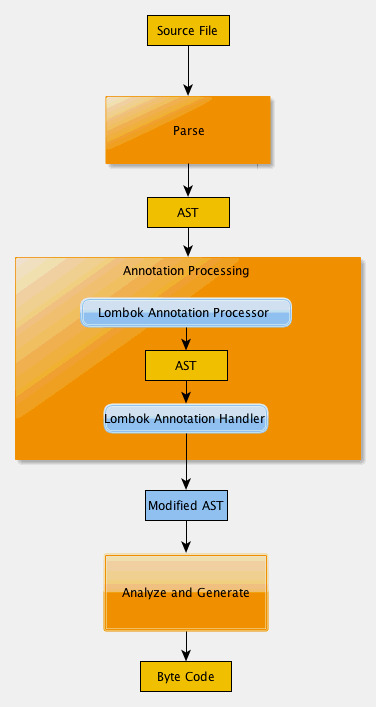
\includegraphics[scale=0.5]{images/lombok.jpg}
    \caption{Lombok Annotation Processor modifies the AST}
    \label{fig:lombok}
\end{figure}

\subsection{@FieldNameConstants annotation}
One of the experimental features of Project Lombok, \texttt{@FieldNameConstants}\footnote{\url{https://projectlombok.org/features/experimental/FieldNameConstants}} annotation is used to generate an inner type that contains a string constant representing a field’s name for each field of the annotated type. This annotation is provided with some room for configuration, such as inclusion or exclusion of particular fields, capitalization of generated fields names, the name of the inner generated type, etc.

Java source with Lombok:
\begin{minted}{java}
@FieldNameConstants
public class Person {
    private String name;
    private int age;
    @FieldNameConstants.Exclude
    private String id;
}
\end{minted}

Equivalent Java source without Lombok:
\begin{minted}{java}
public class Person {
    private String name;
    private int age;
    private String id;

    public static final class Fields {
        public static final String name = "name";
        public static final String age = "age";
    }
}
\end{minted}

This approach, although effective for basic needs, is limited by its simplicity, as indicated by the following points:
\begin{itemize}
    \item The generated entity graph is limited by a depth of a single level, as the generated fields are always of type String.
    \item Domain discoverability is limited by the lack of descriptiveness of the generated fields, since no javadoc accompanying a field is generated.
\end{itemize}

However, the approach employed by Project Lombok is certainly a unique and inspiring piece of work to learn from.

\section{Hibernate Metamodel Generator}

Hibernate is an implementation for the JPA\footnote{Java Persistence API (renamed to Jakarta Persistence)}.

\n

Hibernate Metamodel Generator\footnote{\url{https://docs.jboss.org/hibernate/orm/6.0/topical/html\_single/metamodelgen/MetamodelGenerator.html}} is an annotation processing tool that is a part of the Hibernate ORM framework. It automates the generation of static entity meta-models used for typesafe Criteria queries as defined by the JPA 2. The queries benefit from the meta-models by being able to be constructed in a strongly-typed manner, thus avoiding the risks of type casting the result of a query.

\begin{minted}{java}
@Entity
public class Order {
    @Id
    private long id;

    @ManyToOne
    private Person customer;

    @OneToMany
    private Set<Item> items;

    private BigDecimal totalCost;
}

@StaticMetamodel(Order.class)
public abstract class Order_ {

    public static volatile SingularAttribute<Order, Long> id;
    public static volatile SetAttribute<Order, Item> items;
    public static volatile SingularAttribute<Order, BigDecimal> totalCost;
    public static volatile SingularAttribute<Order, Person> customer;

    public static final String ID = "id";
    public static final String ITEMS = "items";
    public static final String TOTAL_COST = "totalCost";
    public static final String CUSTOMER = "customer";

}

\end{minted}

What stands out is that, apart from the property names, the generated meta-model also captures information about property types, providing an ability to use them in a compile time safe manner. However, since this tool was specifically designed to assist with constructing Criteria queries, its area of application is to some extent bound to the JPA specifications. More specifically, those members of the generated meta-model that capture the property type as a generic type parameter (the first four in the example) are a part of the JPA, hence the tightly coupled implementation.

\n

The major limitation of Hibernate meta-models is that their use for other, JPA unrelated, purposes will most likely end up being as effective as the previously mentioned approach of Project Lombok, thus being subject to the same constraints.


%\end{relatedwork}

\chapter{Implementation details}

The meta-model generation mechanism is implemented as an annotation processor, hereafter referred to as "domain-model processor".

\begin{figure}[H]\centering
    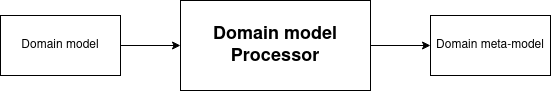
\includegraphics[scale=0.65]{images/implement1.drawio.png}
    \caption[Input and output of the annotation processor]{Annotation processor accepts a processing environment on input and produces generated sources on output}\label{fig:implement1}
\end{figure}

The annotation processor is initialized with a processing environment, by the compiler.
The processing environment provides an AST that was obtained by parsing source files.
In the incremental compilation environments, the processor benefits from the fact that it is possible to access the AST of a source file that was not necessarily a part of the compiler’s input.

\section{Entity graph}
A convenient and intuitive model for entities and their properties is a graph.
The structure of an entity can be represented as a directed graph where each node is a type, with the \textit{source} being the type of the entity itself.
A domain graph must include all entity nodes, thus it may have multiple sources.
An arc $(x, y)$ can be read as "Entity $x$ has a property of type $y$". 

\n

Figure \ref{fig:entity-graph} depicts a graph for entity \texttt{Person}, \texttt{User} and \texttt{Vehicle}.
The labels attached to arcs are the corresponding names of those properties.
All nodes are labeled with their type’s name.
The ones filled with blue are entity types, while those filled with white, which are always sinks, are non-entity types.
An entity graph might contain a cycle.
For example, the above graph contains one cycle $(User, User)$ at the \texttt{basedOnUser} property.

\begin{figure}[H]\centering
    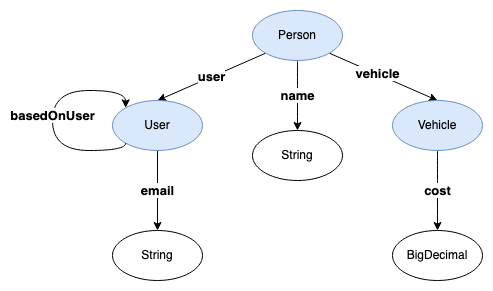
\includegraphics[scale=0.65]{images/entity-graph.drawio.png}
    \caption{\texttt{Person} entity graph}\label{fig:entity-graph}
\end{figure}

\section{Meta-model generation algorithm}
At the highest level the meta-model generation mechanism functions according to the following rules:
\begin{itemize}
    \item For each class annotated with \texttt{@MapEntityTo} or \texttt{@DomainEntity} there will be a meta-model generated that captures all of its properties, that is, all fields annotated with \texttt{@IsProperty}.
    \item A meta-models collection class will be generated. This class is a container storing an instance of every active meta-model in a static field. In other words, it contains an entity graph for each domain entity.
    \item Whenever a domain entity is modified, the whole entity graph is considered for regeneration. That is, each node representing a domain entity will have its metamodel regenerated. The renaming and deletion of an entity is also covered.
    \item If an entity should no longer be metamodeled, that is, it is either no longer annotated with the above mentioned annotations or deleted, then its meta-model is regenerated into an inactive one. Its entity graph is removed from the meta-models collection class.
\end{itemize}


\begin{figure}[H]\centering
    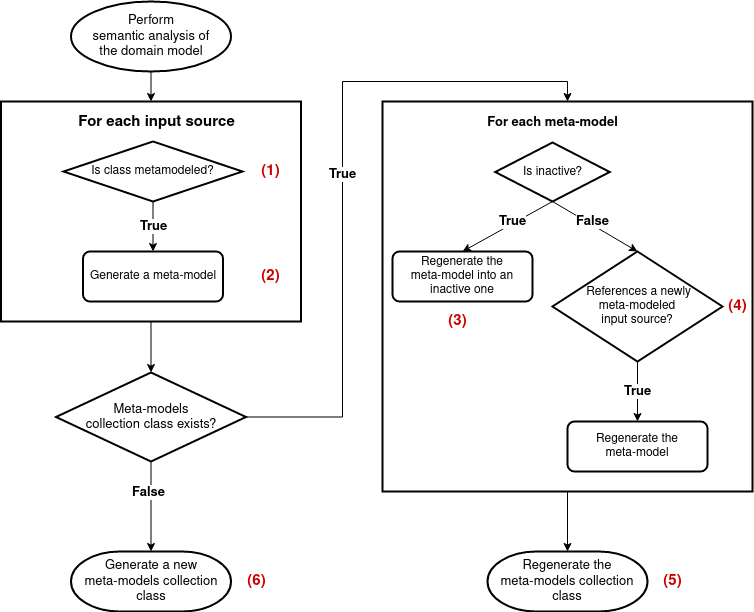
\includegraphics[scale=0.55]{images/algorithm.drawio.png}
    \caption{A high-level view of the meta-model generation algorithm}\label{fig:algorithm}
\end{figure}

\begin{enumerate}[label={\textbf{(\arabic*)}}]
    \item A class is considered to be metamodeled if it’s annotated with \texttt{@MapEntityTo} or \texttt{@DomainEntity}.
    \item This step is illustrated in detail by \ref{fig:meta-model_algorithm}. See \textbf{(2)*}
    \item A meta-model is considered to be inactive if its underlying entity no longer qualifies for being metamodeled. An inactive meta-model is structured in such a way that it effectively becomes "useless". To achieve this in Java we generate an abstract empty class (with no members). The fact that the class is abstract means that it cannot be instantiated. The reasoning behind this choice was to overcome the limitations of an inability to support deletion of meta-models.
    \item In case an entity becomes metamodeled, it is necessary to connect its meta-model to any existing ones, the underlying entities of which are adjacent in the entity graph. In other words, this step is responsible for connecting the entity graphs. This step is discussed in more detail below (\ref{fig:meta-model_graph}). See \textbf{(4)*}.
    \item The meta-models collection class is regenerated by removing fields with inactive meta-models and adding fields for newly generated meta-models if needed.
    \item This step is equivalent to \textbf{(5)}, except that there are no inactive meta-models, since the collection class does not yet exist.
\end{enumerate}

\begin{enumerate}[label={\textbf{(\arabic*)*}}]
\setcounter{enumi}{1}
    \item \;
        \begin{figure}[H]\centering
            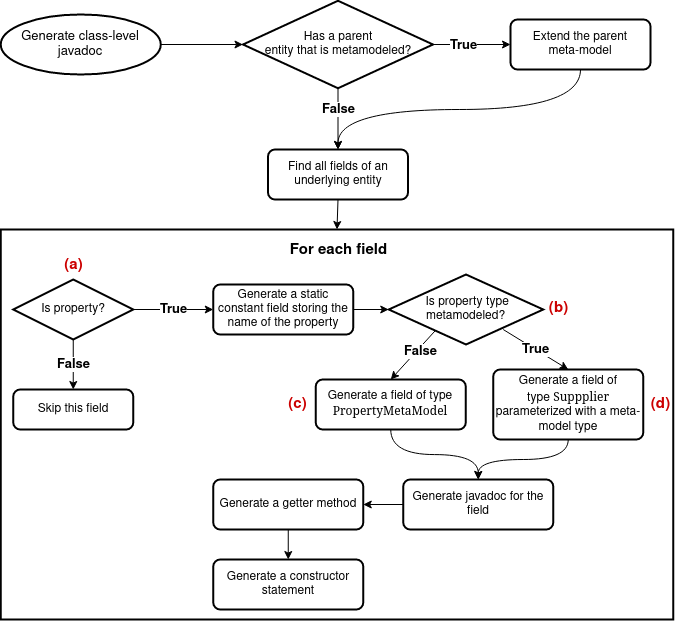
\includegraphics[scale=0.55]{images/meta-model-algorithm.drawio.png}
            \caption{The procedure of generating a meta-model}\label{fig:meta-model_algorithm}
        \end{figure}

        \begin{enumerate}[label={\textbf{(\alph*)}}]
            \item Each field annotated with \texttt{@IsProperty} is considered to be a property of an entity.
            \item See \textbf{(1)} above.
            \item \texttt{PropertyMetaModel} class is used to represent any property that is a sink in the entity graph.
            \item \texttt{Supplier<T>} is a parameterized type used to represent any node in a graph that is not a sink, where \texttt{T} is a meta-model class. This particular type is used in order to achieve lazy computation of an entity node value, since an entity graph may contain a cycle.
        \end{enumerate}

    \addtocounter{enumi}{1}
    \item Consider a situation where \texttt{Person} and \texttt{User} entities are metamodeled, while the \texttt{Vehicle} entity is not. Then the following meta-model graph exists:


        \begin{figure}[H]\centering
            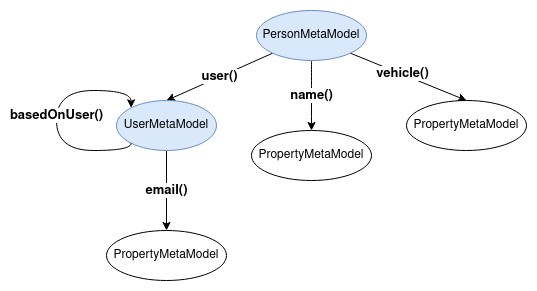
\includegraphics[scale=0.65]{images/meta-model-graph.drawio.png}
            \caption{A meta-model graph for entity \texttt{Person,} where \texttt{User} is metamodeled, but \texttt{Vehicle} is not}\label{fig:meta-model_graph}
        \end{figure}

    Then, if the entity \texttt{Vehicle} becomes metamodeled, the arc $(PersonMetaModel, PropertyMetaModel)$ labeled \texttt{vehicle()} should be replaced by an arc $(PersonMetaModel, VehicleMetaModel)$, effectively connecting both graphs.


        \begin{figure}[H]\centering
            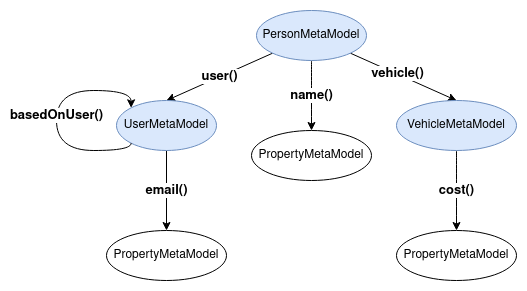
\includegraphics[scale=0.65]{images/meta-model-graph1.drawio.png}
            \caption{A meta-model graph for entity \texttt{Person} after \texttt{Vehicle} was metamodeled}\label{fig:meta-model_graph1}
        \end{figure}

    This can be achieved only by traversing each entity graph in order to find the appropriate adjacent entity nodes ($(Person, Vehicle)$ in the example above).
\end{enumerate}

\section{Meta-model structure}

The following UML class diagram illustrates the structure of the generated meta-models for entities from the example in \ref{fig:entity-graph}.

\begin{figure}[H]\centering
    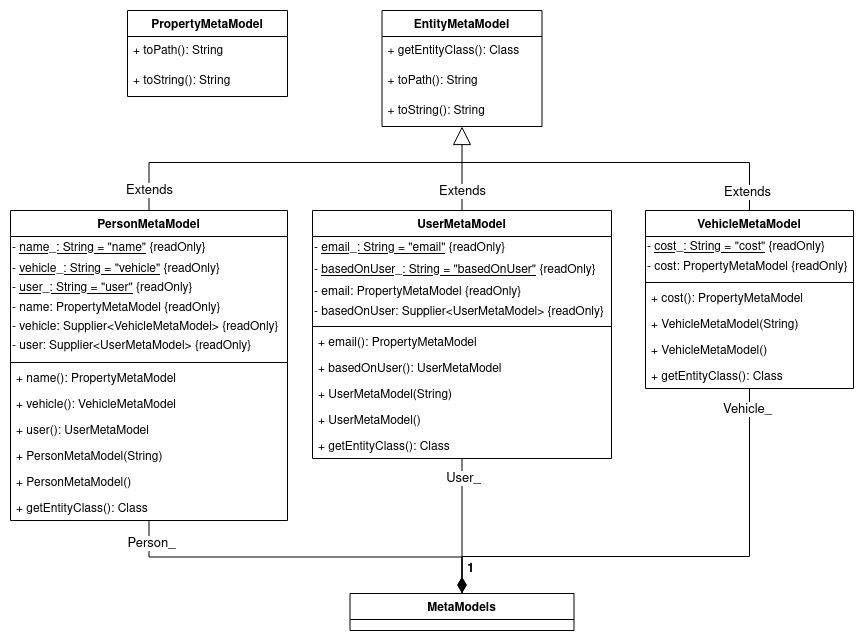
\includegraphics[scale=0.55]{images/meta-model-uml.drawio.png}
    \caption[UML class diagram for generated meta-models]{UML class diagram describing the generated meta-models for the domain illustrated in Figure \ref{fig:entity-graph}}\label{fig:meta-model_uml}
\end{figure}

The actual \texttt{String} value representing the property dot-notation is accessed by calling the \texttt{toPath()} method (or the equivalent \texttt{toString()}). 
A meta-model also implements a \texttt{getEntityClass()} method that can be used to obtain the class of its underlying entity.
Fields of the meta-models collection class (\texttt{MetaModels}) are named by appending the underscore to the name of the underlying entity in order to avoid conflicts that might be caused by static imports in Java (\texttt{Person} as type and \texttt{Person} as statically imported field).
Methods of a meta-model that are used to traverse the entity graph contain additional information about the modeled properties in the form of javadoc as illustrated below:

\n

\begin{listing}[H]
    \begin{minted}{java}
    @IsProperty
    @Title("Name", desc = "The name of this person")
    @MaxLength(255)
    private String name;
    \end{minted}
    \caption{An arbitrary non-entity type property (a sink node in the graph)}
    \label{lst:prop-sink}
\end{listing}

\begin{listing}[H]
    \begin{minted}{java}
    /**
    * Title: Name
    * Description: The name of this person
    * Type: {@link String}
    * {@literal @}{@link IsProperty}
    * {@literal @}{@link MaxLength}(value = 255)
    */
    public PropertyMetaModel name() {
        return this.name;
        }
    \end{minted}
    \caption{A property metamodeled after \ref{lst:prop-sink}}
    \label{lst:meta-prop-sink}
\end{listing}

\begin{listing}[H]
    \begin{minted}{java}
    @IsProperty
    @Title("User", desc = "User associated with this person")
    private User user;
    \end{minted}
    \caption{An arbitrary entity-type property}
    \label{lst:prop-entity}
\end{listing}

\begin{listing}[H]
    \begin{minted}{java}
    /**
     * Title: User
     * Description: User associated with this person
     * Type: {@link User}
     * Meta-model: {@link UserMetaModel}
     * {@literal @}{@link IsProperty}
     */
    public UserMetaModel user() {
        return this.user.get();
    }
    \end{minted}
    \caption{A property metamodeled after \ref{lst:prop-entity}}
    \label{lst:meta-prop-entity}
\end{listing}


\section{Usage example}
\begin{listing}[H]
    \begin{minted}[linenos]{java}
    public class PersonFetcher {
        static final PersonMetaModel person = MetaModels.Person;
            
        // a fetch model used to fetch data from a database
        static final Fetch<Person> FETCH = fetch(Person.class).with(
                // sink node
                person.name(),                   // "name"

                // entity node
                person.user(),                   // "user"
                person.user().basedOnUser(),     // "user.basedOnUser"
                person.vehicle(),                // "vehicle"
                person.vehicle().cost(),         // "vehicle.cost"

                // source node
                person                           // "this"
                );
    }
    \end{minted}
    \caption{Using the meta-model for entity \texttt{Person} to traverse its graph}
    \label{lst:person_meta-model_usage}
\end{listing}

Suppose that the conceptual schema has changed, resulting in the \texttt{Vehicle} entity no longer having the property \texttt{cost}. Then, the following compilation error would occur at line 13:
\begin{minted}[escapeinside=||]{java}
    // error: The method cost() is undefined for the type VehicleMetaModel
    person.vehicle().|\textcolor{red}{\uwave{\textcolor{black}{cost()}}}|,
\end{minted}

\n

The true power of a meta-model is manifested in combination with code auto-completion:

\begin{figure}[H]\centering
    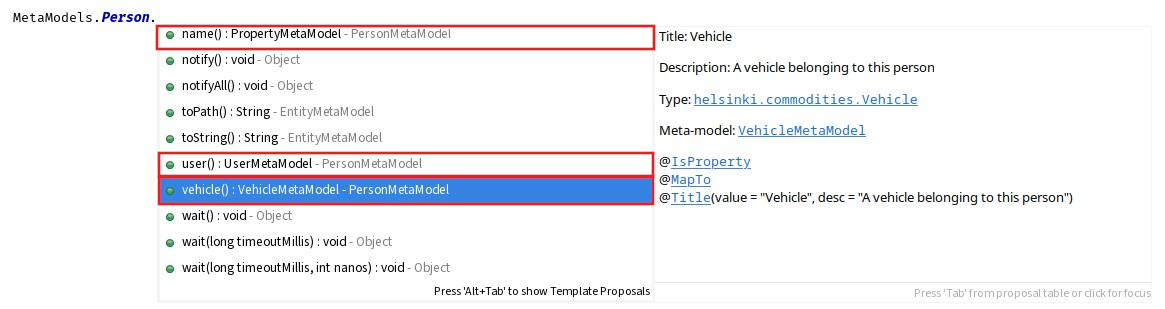
\includegraphics[scale=0.5]{images/eclipse-hl.jpg}
    \caption[Traversing the entity graph with the help of Eclipse IDE code auto-completion feature]{Traversing the entity graph with the help of Eclipse IDE code auto-completion feature
    \\
    \textit{Note}: Property-methods are highlighted}\label{fig:meta-model_uml}
\end{figure}



\chapter{Experiment}

Evaluation of the developed technology was conducted in the form of an experiment.
The motivation behind this choice was the desire to assess the extent to which all stated objectives were reached.
Although, the intuitive choice was to employ an approach of automated software testing, not all objectives could be effectively assessed in that manner.
Domain discoverability, in particular, is better suited to evalutaion by opinion, because of its subjective nature. Also, given rather uncommon software development technique of code generation, as well as the intricate dependencies between the generated and source code, it was challenging to use automated tests for assessment of the other two objectives, namely, model consistency and evolvability. Therefore we use the experiment as a single source of evaluation.

\n

Naturally, given the tight coupling to Trident Genesis, the experiment's audience was comprised of 7 software engineers working on several projects built with TG at their core.
The experiment had been conducted over a period of one week, at the end of which every team member was asked to fill out a questionnaire.
Each individual was asked to agree/disagree with a handful of statements and optionally provide additional comments.

\n

Despite the fact that the actual duration was shorter than originally planned, most answers convey enough information with only a few where several respondents share the opinion that more time is required. 
What follows is a display of responses, accompanied by several selected comments that contributed valuable insight.

\section{Discoverability of the domain model}

\mychart{5}{2}{0}{0}{0}{Question 1: Domain discoverability}{The information provided by meta-models in the form of javadoc combined with the IDE’s code auto-completion feature made domain discoverability more efficient.}

\mychart{5}{2}{0}{0}{0}{Question 2: Domain discoverability}{When attempting to refer to a property of an entity using a meta-model, there was no need for context switching, i.e., opening an entity class and looking for the property definition.}

\mychart{0}{2}{3}{1}{1}{Question 3: Domain discoverability}{The generated meta-models could contain more information about their underlying entities.}

\section{Reliability}

\mychart{4}{3}{0}{0}{0}{Question 4: Reliability}{Usage of the generated meta-models proved to be a reliable way of referencing properties of an entity, i.e., there were no occurrences of runtime errors.}

\section{Evolvability}

\mychart{4}{2}{1}{0}{0}{Question 5: Evolvability}{Evolvability of a system against modifications to the conceptual model increased due to compile-time validation in places where the generated meta-models were referenced.}

\section{Performance}

\mychart{5}{2}{0}{0}{0}{Question 6: Performance}{Impact of the meta-model generation process on performance of the IDE during compilation has been insignificant to the development process.}

\section{Correctness of the generation mechanism}
\mychart{4}{2}{1}{0}{0}{Question 7: Correctness}{The meta-model generation mechanism was always correctly generating meta-models for newly added entities.}

\mychart{4}{2}{1}{0}{0}{Question 8: Correctness}{The meta-model generation mechanism was acting correctly in response to the renaming / deletion of an entity.}

\mychart{5}{2}{0}{0}{0}{Question 9: Domain discoverability}{The meta-model generation mechanism was always correctly adapting the latest modifications to the conceptual model.}

\section{Intuitiveness and ease of use}
\mychart{5}{2}{0}{0}{0}{Question 10: Intuitiveness and ease of use}{Overall structure of the entity meta-model was easy to understand and intuitive in its use for referencing and chaining properties of an entity.}

\mychart{0}{1}{5}{0}{1}{Question 11: Intuitiveness and ease of use}{The entity meta-model could be structured in a better way.}

\mychart{5}{2}{0}{0}{0}{Question 12: Intuitiveness and ease of use}{Overall, I am rather satisfied with the experience of utilizing the meta-model generation tool.}

\chapter{Future work}


%----------------------------------------------------------------------------------------
%	THESIS CONTENT - APPENDICES
%----------------------------------------------------------------------------------------

\appendix % Cue to tell LaTeX that the following "chapters" are Appendices

% Include the appendices of the thesis as separate files from the Appendices folder
% Uncomment the lines as you write the Appendices

%\include{Appendices/AppendixA}
%\include{Appendices/AppendixB}
%\include{Appendices/AppendixC}

%----------------------------------------------------------------------------------------
%	BIBLIOGRAPHY
%----------------------------------------------------------------------------------------
\printbibliography[heading=bibintoc]

%----------------------------------------------------------------------------------------

\end{document}  
